% : Fast and Effective Binary for WebAssembly
\msection{Wasm-mutate}
\renewcommand{\tool}{wasm-mutate\xspace}

In this section we present \tool, a tool to diversify
WebAssembly binaries and produce semantically equivalent variants.
\tool is highlighted as the blue squared tooling in \autoref{fig:approach_landscape}.
The primary objective of \tool is to generate semantically equivalent variants from a given WebAssembly binary input. 
\tool's central approach involves synthesizing these variants by substituting parts of the original binary using rewriting rules. 
It leverages a comprehensive set of rewrite rules, boosted by a diversification space traversals using e-graphs \cite{egraph}.

\begin{figure*}[h!]
    \centering
    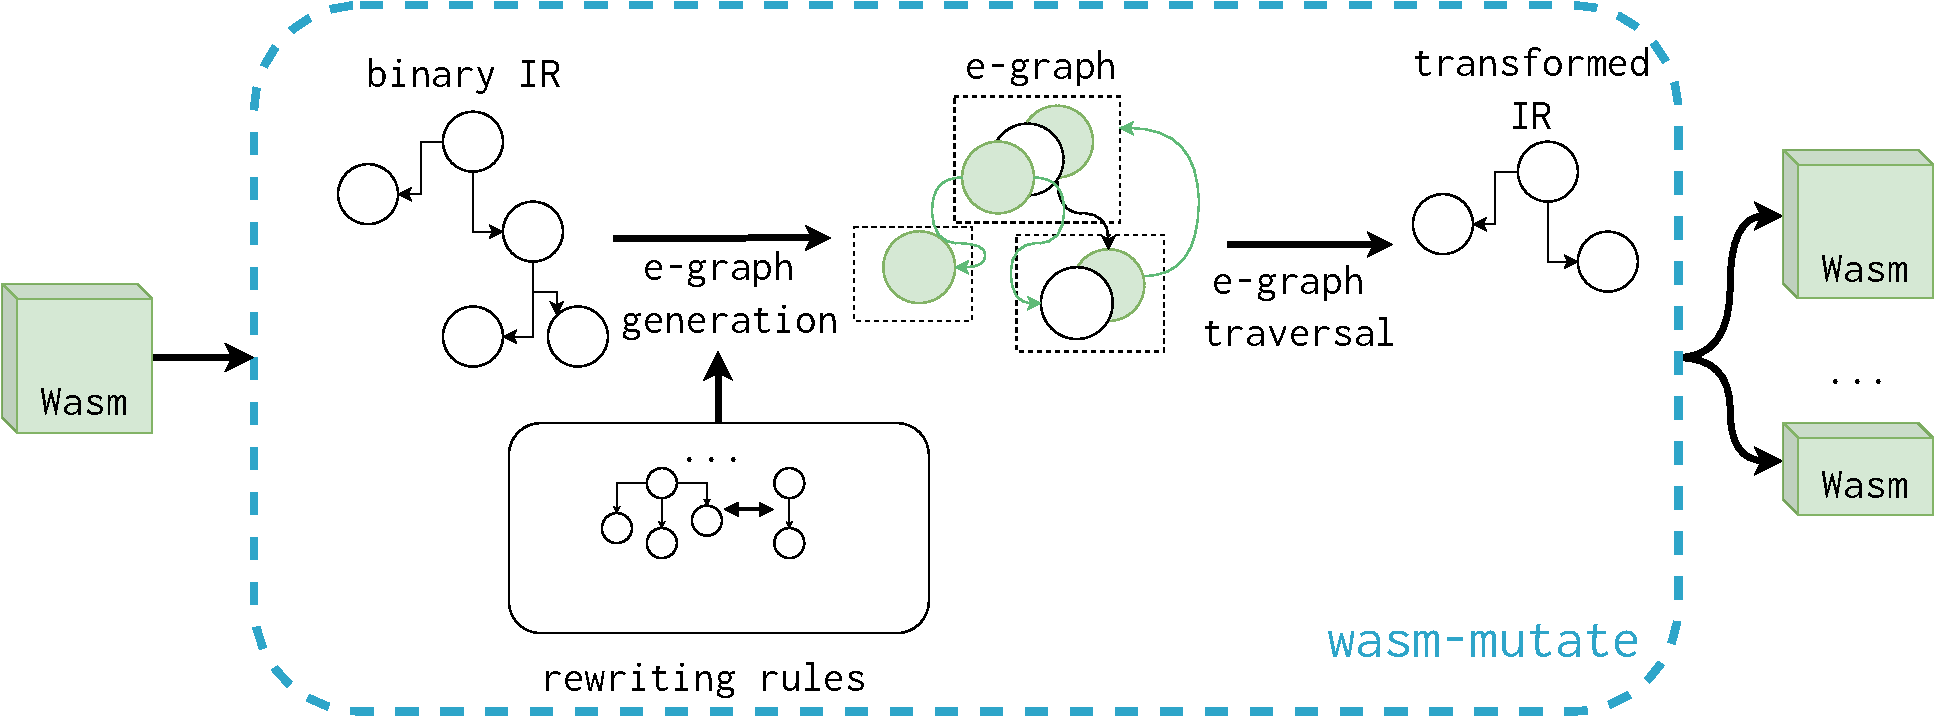
\includegraphics[width=0.9\linewidth]{diagrams/wasm_mutate.workflow.pdf}
    \caption{ \tool high level architecture.  It generates semantically equivalent variants from a given WebAssembly binary input. 
    Its central approach involves synthesizing these variants by substituting parts of the original binary using rewriting rules, boosted by a diversification space traversals using e-graphs(refer to \autoref{alg}).}
  \label{fig:wasm-mutate}
\end{figure*}


\autoref{fig:wasm-mutate} illustrates the workflow of \tool, which initiates with a WebAssembly binary as its input. 
The first step involves parsing this binary to create suitable abstractions, e.g., data flow graphs.
Subsequently, \tool utilizes predefined rewriting rules to construct an e-graph for the initial program, encapsulating all potential equivalent codes derived from the rewriting rules. 
This stage exploits an essential e-graph property: each path traversed within the e-graph yields semantically equivalent code.
Then, pieces of the original program are randomly substituted by the result of random e-graph traversals, resulting in a variant that maintains semantic equivalence to the original binary. 
This assurance of semantic preservation is rooted in the inherent properties of the individual rewrite rules employed.
Notice that, the output of \tool can be used back as an input, facilitating the stacking of multiple transformations through repeated \tool iterations.


%% Move this to the new in practice section


%\begin{figure}[h!]
%    \centering
%    \includegraphics[width=.8\linewidth]{figures/process.pdf}
%    \caption{}
%  \label{fig:wasm-mutate-process}
%\end{figure}




\msubsection{WebAssembly Rewriting Rules}
\tool incorporates a total of 135 rewriting rules, organized into categories referred to as meta-rules. 
A significant portion of these, 125 to be exact, fall under a peephole meta-rule.
The rewriting rules are conceived based on the seminal work of Sasnauskas et al. \cite{2017arXiv171104422S}, extended to include a predicate to enforce the conditions for replacement. 
Each rule is articulated as a tuple, represented as \texttt{(LHS, RHS, Cond)}, where: \texttt{LHS} identifies the segment of code targeted for replacement, \texttt{RHS} outlines the functionally equivalent substitute, and \texttt{Cond} defines the circumstances permitting the substitution.
For example, in the case of \Wasm binaries, the \texttt{Cond} predicate ensures that the replacement does not violate the type constraints of the \texttt{part}. 
The following text details seven prominent meta-rules utilized in \tool.

%% Move to Discussion

%We make emphasis on crafting rules that ensure functional equivalence, meaning the programs variants, generated by \too, maintain the same input-output relationship.
%


\wrule{Add type:}
%% This will come in the Background section
%In WebAssembly, the type section wraps definitions of signatures for the binary functions.
\tool implements two rewrite rules for the Type Section of input \Wasm programs, one of which is illustrated in the following rewriting rule. 

\begin{minipage}{0.9\linewidth}
  
{\footnotesize
\lstdefinestyle{watcode}{
  numbers=none,
  stepnumber=1,
  numbersep=10pt,
  tabsize=4,
  showspaces=false,
  breaklines=true, 
  showstringspaces=false,
    moredelim=**[is][{\btHL[fill=weborange!40]}]{`}{`},
    moredelim=**[is][{\btHL[fill=celadon!40]}]{!}{!},
    moredelim=**[is][{\btHL[fill=frenchplum!40]}]{bb}{bb},
    moredelim=**[is][{\btHL[fill=eminence!40]}]{bc}{bc}
}

\lstset{
        language=ttt,
        style=watcode,
        basicstyle=\footnotesize\ttfamily,
        columns=fullflexible,
        breaklines=true}
\begin{lstlisting}[numbers=none]{Name}
LHS (module
  (type (;0;) (func (param i32) (result i64)))
        \end{lstlisting}  
\hrulefill

\begin{lstlisting}[numbers=none]{Name}
RHS (module
  (type (;0;) (func (param i32) (result i64)))
!+ (type (;0;) (func (param i64) (result i32 i64)))!
        \end{lstlisting}   
}
\vspace{2mm}
\end{minipage}

This transformation generates random function signatures with a random number of parameters and results count.
This rewriting rule does not affect the runtime behavior of the  variant.
It also guarantees that the index of the already defined types is consistent after the addition of a new type. 
%% This will come in the background section
% This is because Wasm programs cannot access or use a type definition during runtime, they are only used to validate the signature of a function during compilation and validation from the host engine.
%% This is for the evaluation part
%From the security perspective, this transformation prevents against static binary analysis. 
%For example, to avoid malware detection based on signature set \cite{CABRERAARTEAGA2023103296}.

\wrule{Add function:} The function and code sections of a Wasm binary contain function  declarations and the code body of the declared functions, respectively.
\tool add new functions, through mutations in the two mentioned sections.
To add a new function, \tool creates a random type signature.
Then, the random function body is created.
The body of the function consists of returning the default value of the result type.
\tool never adds a call instruction to this function.
So in practice, the new function is never executed.
The following example illustrates this rewriting rule.

\begin{minipage}{0.9\linewidth} 
    
\lstdefinestyle{watcode}{
    numbers=none,
    stepnumber=1,
    numbersep=10pt,
    tabsize=4,
    showspaces=false,
    breaklines=true, 
    showstringspaces=false,
      moredelim=**[is][{\btHL[fill=black!10]}]{`}{`},
      moredelim=**[is][{\btHL[fill=celadon!40]}]{!}{!}
  }
  
  {
  \captionsetup{width=\linewidth}
  \noindent\begin{minipage}[b]{\linewidth}
      \lstset{
          language=ttt,
          style=watcode,
          basicstyle=\footnotesize\ttfamily,
          columns=fullflexible,
          breaklines=true}
          \begin{lstlisting}[]{Name}
   LHS (module
      (type (;0;) (func (param i32 f32) (result i64)))
          \end{lstlisting}
          %\vspace{0.2cm}
     \end{minipage}
     
  \noindent\hrulefill
  
  \noindent\begin{minipage}[b]{\linewidth}
      \lstset{
          language=ttt,
          style=watcode,
          basicstyle=\footnotesize\ttfamily,
          columns=fullflexible,
          breaklines=true}
          \begin{lstlisting}[]{Name}
   RHS (module
      (type (;0;) (func (param T) (result t)))
      (func (;0;) (type 0) (param T) (result t)
         t.const 0) 
          \end{lstlisting}
          %\vspace{0.2cm}
     \end{minipage}
     
  }
  
\end{minipage}

%% This is for the discussion section. Where we compare the type of transformations, the tools, and the security impact.
%Therefore, executing both, the original binary and the mutated one with the same input, lead to the same final state.
%This strategy follows the work of Cohen, advocating the insertion of harmless `garbage' code into a program. 
%These transformations do not impact the program's functionality; its increases its static complexity.

\wrule{Remove dead code:} \tool can randomly remove dead code.
In particular \tool removes: \emph{functions, types, custom sections, imports, tables, memories, globals, data segments and elements} that can be validated as dead code.
For instance, to delete a memory declaration, the binary code must not contain a memory access operation. 
Separate mutators are included within \tool for each of the aforementioned elements.
For a more concrete example, the following listing illustrates the case of a function removal.

\begin{minipage}{0.9\linewidth} 

\lstdefinestyle{watcode}{
  numbers=none,
  stepnumber=1,
  numbersep=10pt,
  tabsize=4,
  showspaces=false,
  breaklines=true, 
  showstringspaces=false,
    moredelim=**[is][{\btHL[fill=weborange!40]}]{`}{`},
    moredelim=**[is][{\btHL[fill=celadon!40]}]{!}{!}
}

{
    \lstset{
        language=ttt,
        style=watcode,
        basicstyle=\footnotesize\ttfamily,
        columns=fullflexible,
        breaklines=true}
         
\vspace{8mm}
        \begin{lstlisting}[]{Name}
LHS (module (type (func)))
        \end{lstlisting}
\noindent\hrulefill
    \lstset{
        language=ttt,
        style=watcode,
        basicstyle=\footnotesize\ttfamily,
        columns=fullflexible,
        breaklines=true}
        \begin{lstlisting}[numbers=none]{Name}
RHS `- (module (import "" "" (func)))`
        \end{lstlisting}

\lstset{
        language=ttt,
        style=watcode,
        basicstyle=\footnotesize\ttfamily,
        columns=fullflexible,
        breaklines=true}
        \begin{lstlisting}[numbers=none]{Name}
Cond The removed function is not called, it is not exported, and it is not in the binary _table.
        \end{lstlisting}
}
\end{minipage}

When removing a function, \tool ensures that the resulting binary remains valid and semantically identical to the original binary: it checks  that the deleted function was neither called within the binary code nor exported in the binary external interface. 
As exemplified above, \tool might also eliminate a function import while removing the function. 

%% This comes for the discussion part
%Eliminating dead code serves a dual purpose: it minimizes the attack surface available to potential malicious actors \cite{236200} and strengthens the resilience of security protocols. 
%For instance, it can obstruct signature-based identification \cite{CABRERAARTEAGA2023103296}.
%With Narayan and colleagues having demonstrated the feasibility of Return-Oriented Programming (ROP) attacks \cite{Swivel}, the removal of dead code is able to stop jumps to harmful behaviors within the binary. 
%On the other hand, the act of removing dead code  reduces the binary's size, improving its non-functional properties, in particular bandwidth constraints. 


\wrule{Edit custom sections:}
The custom section in WebAssembly is used to store metadata, such as the name of the compiler that produces the binary or the symbol information for debugging.
%% Move to discussion table
%Thus, this section does not affect the execution of the Wasm program.
\tool includes one mutator to edit custom sections. 
This is exemplified in the following rewriting rule. 

\begin{minipage}{0.9\linewidth} 

\lstdefinestyle{watcode}{
  numbers=none,
  stepnumber=1,
  numbersep=10pt,
  tabsize=4,
  showspaces=false,
  breaklines=true, 
  showstringspaces=false,
    moredelim=**[is][{\btHL[fill=weborange!40]}]{`}{`},
    moredelim=**[is][{\btHL[fill=celadon!40]}]{!}{!}
}

{
    \lstset{
        language=ttt,
                        style=watcode,
        basicstyle=\footnotesize\ttfamily,
                        columns=fullflexible,
                        breaklines=true}
        
        \begin{lstlisting}[]{Name}
LHS (module
...
    `-    (@custom "CS42" "zzz..."`
        \end{lstlisting}
\noindent\hrulefill
        
{
    \lstset{
        language=ttt,
                        style=watcode,
        basicstyle=\footnotesize\ttfamily,
                        columns=fullflexible,
                        breaklines=true}
        
        \begin{lstlisting}[]{Name}
RHS (module
...
    !+    (@custom "CS42" "xxx...")!
        \end{lstlisting}
}
}
\end{minipage}
        

The \emph{Edit Custom Section} transformation operates by randomly modifying either the content or the name of the custom section. 

%% This goes to the discussion part
%As illustrated by Cabrera-Arteaga et al. \cite{CABRERAARTEAGA2023103296}, such a rewriting strategy also acts as a potent deterrent against compiler identification techniques.
% Furthermore, it can also be employed in an innovative manner to emulate the characteristics of a different compiler, \emph{masquerading} as another compilation source. 
% This strategy ultimately aids in shrinking the identification and fingerprinting surface accessible to potential adversaries, hence enhancing overall system security, or to make it a moving target.



\wrule{If swapping:} In WebAssembly, an if-construction consists of a consequence and an alternative. The branching condition is executed right before the \texttt{if} instruction; if the value at the top of the execution stack is greater than \texttt{0}, then the consequence-code is executed, otherwise the alternative-code is run.
The \emph{if swapping} rewriting swaps the consequence and alternative codes of an if-construction.

%% For the discussion part
% This strategy has been employed in other software stacks as well.
% This strategy increases the difficulty for an attacker to predict the program's control-flow, making it more challenging to exploit vulnerabilities.

% https://ieeexplore.ieee.org/document/6915508
% Protecting JavaScript Apps from Code Analysis
% Composite Software Diversification

To swap an if-construction in WebAssembly, \tool inserts a negation of the value at the top of the stack right before the \texttt{if} instruction.
In the following rewriting rule we show how \tool performs this rewriting.

\begin{minipage}{0.9\linewidth} 

\lstdefinestyle{watcode}{
  numbers=none,
  stepnumber=1,
  numbersep=10pt,
  tabsize=4,
  showspaces=false,
  breaklines=true, 
  showstringspaces=false,
    moredelim=**[is][{\btHL[fill=weborange!40]}]{`}{`},
    moredelim=**[is][{\btHL[fill=celadon!40]}]{!}{!},
    moredelim=**[is][{\btHL[fill=frenchplum!40]}]{bb}{bb},
    moredelim=**[is][{\btHL[fill=eminence!40]}]{bc}{bc}
}

{
    \lstset{
        language=ttt,
                        style=watcode,
        basicstyle=\footnotesize\ttfamily,
                        columns=fullflexible,
                        breaklines=true}
        
        \begin{lstlisting}[]{Name}
LHS (module
    (func ...) (
bb condition C bb
        (if bb A bb  else bb  B bb end)
    )
)
        \end{lstlisting}

\noindent\hrulefill


{
    \lstset{
        language=ttt,
                        style=watcode,
        basicstyle=\footnotesize\ttfamily,
                        columns=fullflexible,
                        breaklines=true}
        
        \begin{lstlisting}[]{Name}
RHS (module
    (func ...) (
bb condition C bb
!i32.eqz!
        (if bb B bb else bb A bb end)
    )
)
        \end{lstlisting}

}
}
\end{minipage}
        

\todo{Define if constructions in the Background section.}

The consequence and alternative codes are annotated with the letters \texttt{A} and \texttt{B}, respectively.
The condition of the if-construction is denoted as \texttt{C}.
The negation of the condition is achieved by adding the \texttt{i32.eqz} instruction in the RHS part of the rewriting rule.
The \texttt{i32.eqz} instruction compares the top value of the stack with zero, pushing the value \texttt{1} if the comparison is true.
Some if-constructions may not have either a consequence or an alternative code.
In such cases, \tool replaces the missing code block with a single \texttt{nop} instruction.
%% Move to discussion

% In the context of ROP \cite{Swivel}, this transformation can protect a victim binary to be exploited. 



\wrule{Loop Unrolling:} 
Loop unrolling is a technique employed to enhance the performance of programs by reducing loop control overhead \cite{dongarra1979unrolling}. 
%Although the original functionality of the program remains unchanged, its static structure and performed operations are altered.
\tool incorporates a loop unrolling transformation and utilizes the Abstract Syntax Tree (AST) of the original Wasm binary to identify loop constructions. 

When \tool selects a loop for unrolling, its instructions are divided by first-order breaks, which are jumps to the loop's start. 
This separation ensures that branching instructions controlling the loop body do not require label index adjustments during unrolling. 
The same holds true for instructions continuing to the next loop iteration.
As the loop unrolling process unfolds, a new Wasm block is created to encompass both the duplicated loop body and the original loop. 
Within this newly established block, the previously separated groups of instructions are copied. 
These replicated groups of instructions mirror the original ones, except for branching instructions jumping outside the loop body, which need their jumping indices increased by one. 
This modification is required due to the introduction of a new \texttt{block ... end} scope around the loop body, which affects the scope levels of the branching instructions.
In the following text we illustrate the rewriting rule for a function that contains a loop. 

\begin{minipage}{0.9\linewidth}
    
\lstdefinestyle{watcode}{
  numbers=none,
  stepnumber=1,
  numbersep=10pt,
  tabsize=4,
  showspaces=false,
  breaklines=true, 
  showstringspaces=false,
    moredelim=**[is][{\btHL[fill=weborange!40]}]{`}{`},
    moredelim=**[is][{\btHL[fill=celadon!40]}]{!}{!},
    moredelim=**[is][{\btHL[fill=frenchplum!40]}]{bb}{bb},
    moredelim=**[is][{\btHL[fill=eminence!40]}]{bc}{bc}
}

{
    \lstset{
        language=ttt,
                        style=watcode,
        basicstyle=\footnotesize\ttfamily,
                        columns=fullflexible,
                        breaklines=true}
        
        \begin{lstlisting}[escapechar=?]{Name}
LHS (module
    (func ...) (
        (loop ? ?   bb A bb  br_if 0 ? ? bc B bc end) ? ?
? ?    )
)
        \end{lstlisting}
 \noindent\hrulefill
       
{
    \lstset{
        language=ttt,
                        style=watcode,
        basicstyle=\footnotesize\ttfamily,
                        columns=fullflexible,
                        breaklines=true}
        
        \begin{lstlisting}[escapechar=?]{Name}
RHS (module
    (func ...) (
        (block
            (block bb A' bb ? ? br_if 0 ? ? bc B' bc ? ? br 1  ? ? end) ? ?
            (loop ? ? bb A' bb ? ? br_if 0 ? ? bc B' bc ? ? end) 
        end) 
    )
)
        \end{lstlisting}
}
}

\end{minipage}

The loop in the LHS part features a single first-order break, indicating that its execution will cause the program to continue iterating through the loop. 
The loop body concludes right before the \texttt{end} instruction, which highlights the point at which the original loop breaks and resumes program execution.
Upon selecting the loop for unrolling, its instructions are divided into two groups, labeled \texttt{A} and \texttt{B}. 
As illustrated in the RHS part, the unrolling process entails creating two new Wasm blocks. 
The outer block encompasses both the original loop structure and the duplicated loop body, while the inner blocks, denoted as \texttt{A'} and \texttt{B'}, represent modifications of the jump instructions in groups \texttt{A} and \texttt{B}, respectively.
Notice that, any jump instructions within \texttt{A'} and \texttt{B'} that originally leaped outside the loop must have their jump indices incremented by one. 
This adjustment accounts for the new block scope introduced around the loop body during the unrolling process. 
Furthermore, an unconditional branch is placed at the end of the unrolled loop iteration's body. 
This ensures that if the loop body does not continue, the tool breaks out of the scope instead of proceeding to the non-unrolled loop.

%% For the discussion part
%Loop unrolling enhances resistance to static analysis while maintaining the original performance \cite{10.1145/3453483.3454035}. 
%In particular, Crane et al. \cite{10.1145/2810103.2813682} have validated the effectiveness of adding and modifying jump instructions against Function-Reuse attacks.
%Our rewriting rule has the same advantages, it unrolls loops while 1) incorporating new jumps and 2) editing existing jumps, as it can be observed with the addition of the \texttt{br\_if}, \texttt{end}, and \texttt{br} instructions. 



\wrule{Peephole:} 
This transformation category is about rewriting instruction sequences within function bodies, signifying the most granular level of rewriting. 
We implement 125 rewriting rules for this group in \tool. 
We include rewriting rules that affects the memory of the binary.
For example, we include rewriting rules that creates random assignments to newly created global variables.
For these rules, we incorporate several conditions, denoted by \texttt{Cond}, to ensure successful replacement. 
These conditions can be utilized interchangeably and combined to constrain transformations (see \autoref{alg}).

For instance, \tool is designed to guarantee that instructions marked for replacement are deterministic. 
We specifically exclude instructions that could potentially cause undefined behavior, such as function calls, from being mutated. 
For this rewriting type, \tool only alters stack and memory operations, leaving the control frame labels unaffected.


% The peephole category rewriting rules are meticulously designed and manually verified. 

%% Move to discussion
%An instance of such streamlined transformation can is illustrated in \autoref{rewriting}, \texttt{(\ x\ i32.or\ x, x, \{\})} implies that the \texttt{LHS} 'x' is to be replaced by an idempotent bitwise \texttt{i32.or} operation with itself, in the absence of any specific conditions.
%Therefore, this category continues to uphold the benefits previously discussed under the \emph{Remove Dead Code} category.

%\todo{J: Maybe add here somekind of conclusion about how all RR aim for: security, obfuscation, testing and anti-debugging. WDYT?}

%\msubsection{E-graphs for WebAssembly}
\msubsection{E-graphs traversal for variant generation}
\label{alg}

\todo{TBD maybe is good to move this to the background.}

We build \tool on top of e-graphs \cite{10.1145/3571207}.
% Introduce concepts of node, eclass
An e-graph is a graph data structure utilized for representing rewriting rules. 
In an e-graph, there are two types of nodes: e-nodes and e-classes. 
An e-node represents either an operator or an operand involved in the rewriting rule, while an e-class denotes the equivalence classes among e-nodes by grouping them, i.e., an e-class is a virtual node compound of a collection of e-nodes. 
Thus, e-classes contain at least one e-node.
Edges within the graph establish operator-operand equivalence relations between e-nodes and e-classes.

In \tool, the e-graph is automatically built from a WebAssembly program by analyzing its expressions and operations through its data flow graph.
Then, each unique expression, operator, and operand are transformed into e-nodes.
Based on the input rewriting rules, the equivalent expressions are detected, grouping equivalent e-nodes into e-classes.
During the detection of equivalent expressions, new operators could be added to the graph as e-nodes.
Finally, e-nodes within an e-class are connected with edges to represent their equivalence relationships.
This process is carried out while the e-graph changes with the inclusion of new rewriting rules, i.e., until the equality saturation is meet \cite{equality-saturation}.

\begin{figure}
    \centering
    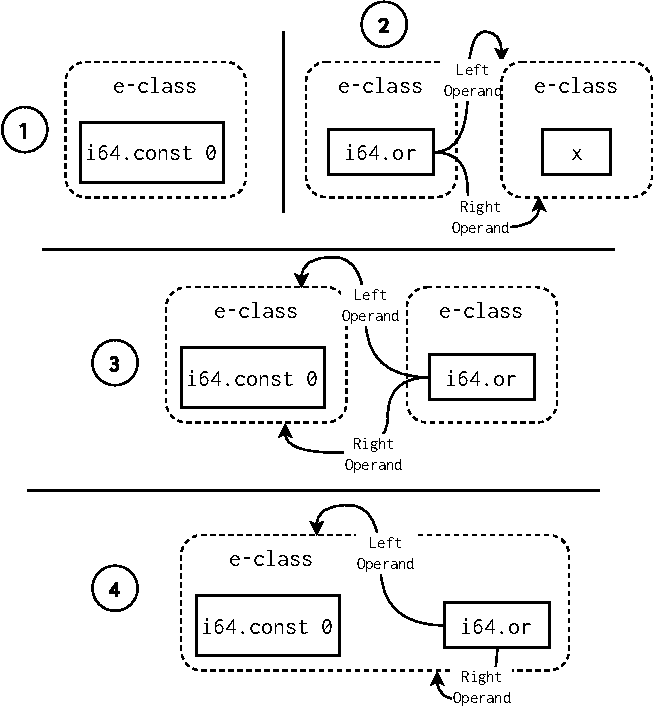
\includegraphics[width=0.5\linewidth]{figures/egraph1.pdf}
    \caption{e-graph for idempotent bitwise-or rewriting rule. Solid lines represent operand-operator relations, and dashed lines represent equivalent class inclusion. }
  \label{e-graph}
\end{figure}

\todo{Expand on e-graphs.}

% How to construct
%% Remove from here
% For example, let us consider one program with a single instruction that returns an integer constant, \texttt{i64.const 0}. Let us also assume a single rewriting rule, \texttt{(x,\ x\ i64.or\ x, x instanceof i64)}. 
% In this example, the program's control flow graph contains just one node, representing the unique instruction.
%The rewriting rule represents the equivalence for performing an \texttt{or} operation with two equal operands.
%\autoref{e-graph} displays the final e-graph data structure constructed out of this single program and rewriting rule. 
%We start by adding the unique program instruction \texttt{i64.const 0} as an en e-node (depicted by the leftmost solid rectangle node in the figure). 
%Next, we generate e-nodes from the rewriting rule (the rightmost solid rectangle) by introducing a new e-node, \texttt{i64.or}, and creating edges to the \texttt{x} e-node.
%Following this, we establish equivalence. 
%The rewriting rule combines the two e-nodes into a single e-class %(indicated by the dashed rectangle node in the figure). 
%As a result, we update the edges to point to the \texttt{x} symbol e-class.


% General use of case
Willsey et al. illustrate that the extraction of code fragments from e-graphs can achieve a high level of flexibility, especially when the extraction process is recursively defined through a cost function applied to e-nodes and their operands. 
This approach guarantees the semantic equivalence of the extracted code \cite{10.1145/3434304}. 
For example, to obtain the smallest code from an e-graph, one could initiate the extraction process at an e-node and then choose the AST with the smallest size from among the operands of its associated e-class \cite{10.1145/3385412.3386012}.

When the cost function is omitted from the extraction methodology, the following property emerges:
\emph{Any path traversed through the e-graph will result in a semantically equivalent code variant}. 
This concept is illustrated in \autoref{e-graph}, where it is possible to construct an infinite sequence of "or" operations.
We leverage this inherent flexibility to generate mutated variants of an original program. 
% How to use it for mutation
The e-graph offers the option for random traversal, allowing for the random selection of an e-node within each e-class visited, thereby yielding an equivalent expression.
%We can extract an infinite number of semantically equivalent expressions from the e-graph, as shown in previous research \cite{10.1145/3571207, 10.1145/3434304}.

%It selects a random instruction within the binary functions and applies one or more of the 125 rewrite rules.
%Finally, it re-encodes the WebAssembly module with the new, rewritten expression to produce a binary variant. 


%\todo{can we make a strong claim here? does everybody maximize simplification with equality saturation? are we the first to do random path in e-grahs?}
We propose and implement an algorithm to randomly traverse an e-graph and generate  semantically equivalent program variants, see \autoref{peephole:mutator}.
It receives an e-graph, an e-class node (initially the root's e-class), and the maximum depth of expression to extract. The depth parameter ensures that the algorithm is not stuck in an infinite recursion. We select a random e-node from the e-class (lines 5 and 6), and the process recursively continues with the children of the selected e-node (line 8) with a decreasing depth. As soon as the depth becomes zero, the algorithm returns the smallest expression out of the current e-class (line 3). The subexpressions are composed together (line 10) for each child, and then the entire expression is returned (line 11). 
To the best of our knowledge, \tool, is the first practical implementation of random e-graph traversal for \Wasm.


\algnewcommand\algorithmicforeach{\textbf{for each}}
\algdef{S}[FOR]{ForEach}[1]{\algorithmicforeach\ #1\ \algorithmicdo}
\begin{algorithm}
    %\footnotesize
	\begin{algorithmic}[1]
	%	\Procedure{MyProcedure}{}
      \Procedure{traverse}{$egraph$, $eclass$, $depth$}
      \\
        \If{depth = 0}
          \State  \Return \textbf{smallest\_tree\_from}(egraph,\ eclass)
        \Else
            \State $nodes \gets egraph[eclass]$
            \State $node \gets random\_choice(nodes)$
            \State $expr \gets (node, operands=[])$
            \ForEach {$child \in node.children $}
                \State $subexpr \gets \textbf{TRAVERSE}(egraph,\ child,\ depth - 1)$
                \State $expr.operands \gets expr.operands \cup\ \{subexpr\}$
            \EndFor
            \State \Return $expr$
        \EndIf
        \EndProcedure
	\end{algorithmic} 
	\caption{e-graph traversal algorithm taken from \cite{wasm-mutate}.} 
	\label{peephole:mutator}
\end{algorithm}

\msubsection{\tool instantiation}

% Example of a random e-graph traversal 
Let us demonstrate how the proposed traversal algorithm can generate program variants with an example. 
We will illustrate Algorithm \ref{peephole:mutator} using a maximum depth of 1. 
\autoref{example:peeporig} presents a hypothetical original Wasm binary to mutate. 
In this example, the developer has established two rewriting rules: \texttt{(x, x i32.or x, x instanceof i32)} and \texttt{(x, x i32.add 0, x instanceof i32)}. The first rewriting rule represents the equivalence of performing an \texttt{or} operation with two equal operands, while the second rule signifies the equivalence of adding 0 to any numeric value.
By employing the code and the rewriting rules, we can construct the e-graph depicted in \autoref{e-graph3}. The figure demonstrates the operator-operand relationship using arrows between the corresponding nodes.


\begin{minipage}[b]{\linewidth}
    \lstset{
        language=WAT,
                        style=watcode,
        basicstyle=\footnotesize\ttfamily,
                        columns=fullflexible,
                        breaklines=true}
        
        \begin{lstlisting}[label=example:peepapplied,caption={Random peephole mutation using e-graph traversal for \autoref{example:peeporig} over e-graph \autoref{e-graph3}. The textual format is folded for better understanding.},frame=b, captionpos=b]{Name}
(module
    (type (;0;) (func (param i32 f32) (result i64)))
    (func (;0;) (type 0) (param i32 f32) (result i64)
        !(i64.add (!
            !i64.const 0!
            !i64.const 1!
            !nop!
        !))!
    )
        \end{lstlisting}
\end{minipage}

\end{minipage}



\begin{figure}
    \centering
    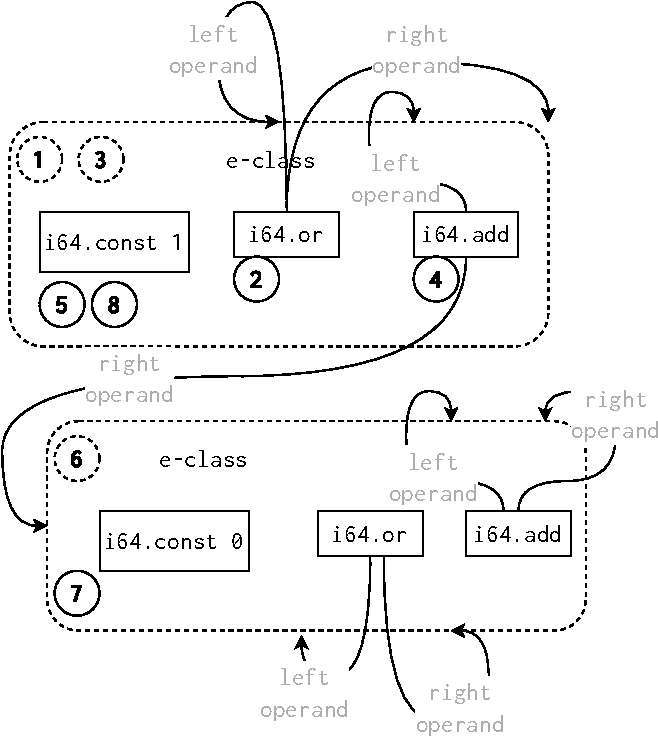
\includegraphics[width=0.75\linewidth]{figures/egraph3.pdf}
    \caption{e-graph built for rewriting the first instruction of \autoref{example:peeporig}. }
  \label{e-graph3}
\end{figure}



In \autoref{e-graph3}, we annotate the various steps of Algorithm \ref{peephole:mutator} 
for the scenario  described above. Algorithm \ref{peephole:mutator} begins at the e-class containing the single instruction \texttt{i64.const 1} from \autoref{example:peeporig}. 
It then selects an equivalent node in the e-class \step{2}, in this case, the \texttt{i64.or} node, resulting in:
{\texttt{expr = i64.or l r}}.
The traversal proceeds with the left operand of the selected node \step{3}, choosing the \texttt{i64.add} node within the e-class: 
{\texttt{expr = i64.or (i64.add l r)} \texttt{r}}.
The left operand of the \texttt{i64.add} node is the original node \step{5}: 
{\texttt{expr = i64.or (i64.add i64.const 1 r)} \texttt{r}}.
The right operand of the \texttt{i64.add} node belongs to another e-class, where the node \texttt{i64.const 0} is selected \step{6}\step{7}:
{\texttt{expr = i64.or (i64.add i64.const 1 i64.const 0)} \texttt{r}}.
In the final step \step{8}, the right operand of the \texttt{i64.or} is selected, corresponding to the initial instruction e-node, returning:
{\texttt{expr = i64.or (i64.add i64.const 1 i64.const 0)\ i64.const 1}}
The traversal result applied to the original Wasm code can observed in \autoref{example:peepapplied}. 


\msubsection{\tool's versatility}

\todo{Custom and abstract rules.}

\todo{Add here other rules. For example global usage}